\lhead{\begin{tikzpicture}[remember picture, overlay]
    \node [anchor=100,inner sep=0] (imagenIZQUIERDA) at (current page header area.north){
\includegraphics[width=18cm]{12/Img/Encabezado.PNG}};
    \end{tikzpicture}}
    \rhead{ García-Hernández}
    \rfoot{\begin{tikzpicture}[remember picture, overlay]
    \node [anchor=140,inner sep=0] (imagenDERECHA) at (current page footer area.south){
\includegraphics[width=18cm]{12/Img/Foot.PNG}};
    \end{tikzpicture}}
    %----------------------------------------------------------------------------------------
    \lfoot{ \thepage}
    % \renewcommand{\labelenumi}{\alph{enumi}.)} 
    %----------------------------------------------------------------------------------------
    %----------------------------------------------------------------------------------------
    %	TITLE SECTION
    %----------------------------------------------------------------------------------------
    
    \setlength{\droptitle}{-5\baselineskip} % Move the title up
    \title{\textbf{Estudio de tiempos y movimientos en el ensamble de un circuito electrónico utilizando diferentes métodos para su optimización }} % Article title
    
     \author{ 
     \textsc{Garcia Hernandez, Pedro Damian}\\ 
    %  Afiliación:
     \texttt{ Instituto Tecnológico de Querétaro} \\ 
     \texttt{Técnologico Nacional de México } \\ 
     \texttt{Querétaro, México}\\ 
     \texttt{pedroghz432@gmail.com} 
     \and 
     \textsc{Ángeles-Hurtado, Luis Alberto}\\ 
    %  Afiliación:
     \texttt{ Instituto Tecnológico de Querétaro } \\ 
     \texttt{ Tecnológico Nacional de México } \\ 
     \texttt{Querétaro, México}\\ 
     \texttt{alb3rt0.ah@gmail.com} 
    }
    
    
    %----------------------------------------------------------------------------------------
    
    % \begin{document}
    
    % Print the title
    \maketitle
    \thispagestyle{fancy}
    
    %----------------------------------------------------------------------------------------
    %	ARTICLE CONTENTS
    %----------------------------------------------------------------------------------------
    
    % \section*{Resumen}
    % \textit{Palabras clave:}
    % El resumen (ancho de página) deberá contener entre 100 y 200 palabras tipo Adobe Devangari 11 puntos.
    
    \begin{abstract}
    \noindent 
    El resumen (ancho de página) deberá contener entre 100 y 200 palabras tipo Adobe Devangari 11 puntos.
    
    \end{abstract}
    % 
    % 
    \textbf{\textit{Palabras clave}}: {First keyword should be the corresponding to the research area according with the authors guide. Maximum of 6 keywords.}
    % \keywords{First keyword should be the corresponding to the research area according with the authors guide. Maximum of 6 keywords.}
    
    \section{Introducción}
    
    % Define estudio de tiempos y movimientos
    % define que es ensamble
    % define que es circuito electronico
    % define el metodo de tiempos predeterminados
    % define optimización
    %\begin{itemize}
    El estudio de movimientos y tiempos es una técnica a desde su creación se a vuelto de vital importancia para gestión de operaciones, principalmente se centra en la medición de los tiempos necesarios para la ejecución de una tarea. así mediante el análisis de dichos procesos se puede determinar el conjunto de técnicas que pueden llevar a la forma mas eficiente de realización.
    
    Esta metodología particularmente es relevante en la industria, donde se llevan a cabo ensamblajes de diferentes componentes que en su conjunto generan un producto, la creciente demanda y competitividad en la industria hace imprescindible que la manufactura se lleve hasta su máxima optimización.
    
    Por consiguiente, en este practica se pretende realizar un análisis sobre el ensamble de un circuito eléctrico de manera practica para así comprender la aplicación de las técnicas de medición de tiempos y movimientos en una situación laboral real.
    
    Según Ovalle, Cárdenas(2016), concluyeron que el estudio de movimientos y tiempos sigue teniendo vigencia en la actualidad en el desarrollo de sistemas eficientes de trabajo, según sus estudios realizados. Así como el cronometro para la medición de de tareas es uno de los mas utilizados.
    Mientras que para Cuevas, González, Torres, Valladares(2021), El estudio de movimientos y tiempos sigue siendo esencial en la actualidad para las empresas, dada la necesidad de optimizar y mejorar los procesos de forma continua. Tambien da la aperturad generar manuales para la capacitación del personal y que su adaptación sea mejor.\cite{REF2}
    
    Por lo tanto, este proyecto busca reafirmar estos conocimientos y demostrar que incluso en la actualidad puede influir de forma imprescindible en los procesos para una correcta aplicación de mejoras en las diferentes áreas productivas. 
    
        %\item Se debe exponer de manera concreta y en lenguaje sencillo : el tema, o lo(s) objeto (s) de estudio. 
        %\item Se deben de mencionar las metodologías más usadas muy brevemente. 
        %\item Se debe de señalar el avance en los últimos años.
        %\item Al final se debe hacer alusión al o lo(s) objetivos del proyecto de investigación.
        %\item Debe de tener Referencias científicas, URL, tesis, etc.
    %\end{itemize}
    \subsection{Definiciones}
    
    \begin{itemize}
        \item Estudio de tiempos y movimientos: Es el análisis de método, materiales, herramientas e instalación utilizada o que se ha de utilizar en la ejecución de un trabajo.
        \item Ensamble: El ensamblaje se refiere al proceso de unir diferentes componentes mediante técnicas manuales o automatizadas que en su conjunto conforman un producto.
         \item Circuito Electrónico: Un circuito electrónico es un sistema compuesto por componentes electrónicos interconectados que trabajan juntos para realizar una función específica. Estos componentes pueden incluir resistencias, capacitores, inductores, transistores, diodos, circuitos integrados, entre otros, (Malvino, A.P., y Bates, J.A. (2006).
         \item Tiempos Predeterminados: El método de tiempos predeterminados es una técnica de estudio de tiempos que se basa en asignar tiempos estándar predefinidos a las diferentes operaciones o movimientos requeridos para llevar a cabo una tarea específica. Estos tiempos están determinados por tablas o catálogos que contienen valores estándar para una amplia gama de actividades y condiciones de trabajo.
         \item Optimización: La optimización se refiere al proceso de hacer que algo sea lo más efectivo, eficiente o funcional posible. En diversos contextos, la optimización implica encontrar la mejor solución posible dentro de ciertos límites o restricciones, ya sea maximizando el rendimiento, minimizando los costos, reduciendo el tiempo necesario para realizar una tarea o mejorando algún otro aspecto deseado
    \end{itemize}
    % 
    % 
    \section{Justificación}
    En la actualidad en la industria se puede percibir el alza en las demandas de producción por lo cual la competitividad en el área de la manufactura es cada vez mas intensa, lo cual obliga a los reclutadores a buscar profesionales que sean capaces de generar sistemas productivos eficientes y llevar a cabo una optimización de manera continua para evitar la disparidad con su competencia.
    
    Dado que la Tecnología cada vez mas se abre paso en la industria para diferentes realizaciones de Actividades en el área productiva, se requiere de un alto conocimiento y competencias que permitan al analista 
    llevar a cabo su deber a pesar de las nuevas tendencias.
    
    Para complementar lo anterior, según Hernández,G.(2022) El futuro del trabajo no se limita simplemente al progreso tecnológico y la creación de nuevas oportunidades laborales. También implica una transformación en la manera en que llevamos a cabo nuestras responsabilidades diarias y en las expectativas que tienen los empleados. La integración de la tecnología en el ámbito empresarial y la evolución de las dinámicas laborales, que abarcan desde los procesos hasta los métodos de trabajo, han generado nuevas perspectivas en relación con el futuro del empleo, que trascienden la mera creación de nuevas posiciones. Un ejemplo de ello es el impacto en las prácticas de contratación de las empresas o en el bienestar de los empleados dentro de los entornos laborales.\cite{REF4}
    
    Mientras que para Content, B.(2024) La revolución digital ha dejado una marca imborrable en el panorama laboral, presentando desafíos y oportunidades sin precedentes tanto para las organizaciones como para sus empleados. En este escenario, la digitalización de procesos emerge como una táctica esencial para maximizar la utilización de recursos, elevar la eficacia y competitividad, y brindar una experiencia superior en productos y servicios a la clientela.
    
    Por otra parte para González, C. (2024)
    El 40 por ciento de los empleados en México están considerando la posibilidad de buscar un nuevo trabajo en el próximo año, mayormente impulsados por el deseo de encontrar condiciones laborales más favorables y un salario más competitivo. Ante esta tendencia, las compañías están centrando sus esfuerzos en retener talento mediante la adopción de medidas como la flexibilidad en el horario laboral y la integración de tecnología.\cite{REF5}
    %\begin{itemize}
        %\item Se debe de describir lo que se requiere, lo que se necesita o lo que se demanda en la actualidad con un enfoque global pero terminar con menciones a temas locales o nacionales.
        %\item Debe de tener Referencias científicas, URL, tesis, etc.
    %\end{itemize}
    % 
    % 
    \section{Descripción del problema}
    Se nos presenta un circuito eléctrico para el cual existe un ensamble, los distintos componentes son independientes de uno de otro, los principales a mencionar son ESP32-C6, LCD 16X2, Potenciómetro de 1k ohm y cables de conexión.
    La idea fundamental consiste en realizar una guía de ensamble por parte el analista que permita al operador realizar la tarea de forma eficiente y sencilla, para esto se llevara a cabo la realización de diferentes ciclos para obtención de tiempos y movimientos.
    
    El problema principal reside en poder determinar la mejor optimización de la secuencia, mediante las técnicas proporcionados de estudio de movimientos y tiempos para la determinación del tiempo productivo. El circuito debe funcionar y realizar su tarea de forma normal.
    
    Según Correa, J.(2015) El estudio del trabajo es uno de los enfoques más convencionales y frecuentes para mejorar la productividad es mediante la implementación de nuevos procedimientos y la adquisición de equipo y maquinaria actualizados. Sin embargo, esta opción implica una inversión significativa de capital, especialmente cuando se recurre a la importación de equipo y maquinaria, lo que puede generar una salida importante de fondos.\cite{REF6}
    %\begin{itemize}
        %\item Se debe describir la desviación o diferencia del ``es'' con respecto al ``debe ser''.
        %\item Se debe hacer alusión a la incógnita científica*.
        %\item Debe de tener Referencias científicas, URL, tesis, etc.
    %\end{itemize}
    
    %\textbf{*La incógnita científica es el elemento cuya solución incrementa el conocimiento científico.}
    % 
    % 
    \section{Fundamentación teórica}
    El estudio de tiempos es una técnica utilizada en la gestión del
    trabajo y la mejora de procesos para medir y analizar el tiempo que
    lleva realizar una tarea específica. Se usa un estudio de movimientos
    para establecer estándares de tiempos. La experiencia ha demostrado
    que ningún individuo puede establecer estándares consistentes.
    Por lo anterior, se utilizan métodos de registros históricos para
    establecer estándares justos. Asimismo, existen diversas técnicas y
    herramientas que se utilizan para lograr este fin, como son el
    cronómetro, sistemas de tiempo determinado, datos estándar,
    fórmulas de tiempo y fórmulas de muestreo. La estandarización con
    precisión aumenta la eficiencia, y los malos conducen a las fallas del
    sistema.
    
    Para Andrade, M., Del Río, A. y Alvear, L.(2019) El estudio de movimientos y tiempos presenta una principal característica que esta metodología radica en lograr un equilibrio efectivo en la línea de producción. Esto significa distribuir el trabajo de manera equitativa entre los distintos operarios, lo que contribuye a una mayor eficiencia y productividad en la planta.\cite{REF7}
    
    Mientras que para Withing, K.(2024) 
    Las habilidades seran mas importantes Según el Informe sobre el Futuro del Empleo, se anticipa que alrededor del 23 por ciento de los puestos de trabajo sufrirán modificaciones en los próximos cinco años. Esto significa que un gran número de individuos deberán transitar de empleos en disminución hacia aquellos que están en ascenso.\cite{REF8}
    
    Otra Opinión es de Ramírez, L., Olguin, I.y Domínguez, L. (2019) La industria 4.0 enfrenta diversos desafíos y consideraciones, como la automatización de los procesos industriales, la gestión de grandes volúmenes de datos, la introducción de robots colaborativos, la integración de dispositivos electrónicos en la producción y la transformación del ambiente organizacional y los modelos laborales. Sin embargo, uno de los mayores desafíos radica en la integración efectiva del factor humano en este contexto altamente tecnológico y automatizado. Aunque puede ser percibido como una amenaza inicialmente, la industria 4.0 también representa una gran oportunidad para la creación de nuevos roles laborales, la especialización de la mano de obra, la formación de trabajadores con habilidades multidisciplinarias y la posibilidad de salarios más competitivos.\cite{REF9}
    
    %Es la parte medular y de mayor discusión, deberá ser la fundamentación de la hipótesis, por tanto se deberá señalar claramente la razón de la suposición y fundamentación de la misma. Únicamente referencias científicas.
    %\begin{itemize}
        %\item Se debe de retomar el tema que se planteo en la introducción, pero ahora profundizando para clarificar la incógnita científica y se pueda plantear la hipótesis.
        %\item Se debe de retomar la descripción del problema, pero ahora a profundidad del (los) objeto(s) de estudio. 
        %\item Se debe de profundizar en las metodologías que se ha usado para el estudio del tema.
        %\item Referencias solo de artículos y libros científicos.
    %\end{itemize}
    % 
    % 
    \section{Hipótesis}
    
    Es la suposición con fundamento científico relativa a la solución del problema, necesidad o de cómo se aprovecha la oportunidad con la incógnita científica y se fundamenta con: 1. Una suposición (en afirmativo o negativo) y ésta deberá vincularse con:
    2. La fundamentación científica que deberá ser precisa 3. Una entidad de comparación para probar la suposición y
    4. La variable con que se califica o cuantifica la comparación o se prueba la hipótesis.
    
    \begin{itemize}
        \item Se debe de identificar claramente la suposición científica
        \item Se debe de identificar claramente el fundamento científico
        \item Se debe identificar claramente la variable de respuesta
        \item Se debe identifican claramente las realidades o modelos contrastantes
        \item Se debe de establecer las variables asociadas, explicativas o que tienen relación funcional con la variable de respuesta
    \end{itemize}
    % 
    % 
    \section{Objetivo}
    
    Diseña, mejora e integra sistemas productivos de bienes y servicios aplicando tecnologías para su optimización.
    
    %\begin{itemize}
        %\item Se debe establecer que se pretende probar la hipótesis
    %\end{itemize}
    
    \subsection{Objetivos específicos }
    \begin{itemize}
    \item Análisis y estudio de los fundamentos necesarios para la realización de la practica. 
        \item Plantear y comprender el problema que se busca resolver con datos estadísticos y teóricos. 
        \item Organizar y identificar los componentes que conforman el circuito eléctrico.
        \item Generar una guía de ensamble que le proporcione al operario las herramientas necesarias para realizar su tarea.
        \item Obtener tiempos de cada uno de los ciclos para generar datos históricos.
        \item Con base a los datos históricos determinar el tiempo productivo y la forma mas eficiente de realizar la tarea. 
    \end{itemize}
    %\begin{itemize}
        %\item Se debe establecer como un conjunto de acciones comunes para lograr el objetivo general
        %\item Se debe establecer como etapas para lograr el objetivo general
    %\end{itemize}
    
    %Son actividades orientadas al cumplimiento del objetivo general. Se establecen con verbos activos en infinitivo. Son parte de la acción encaminada a probar la hipótesis. Éstos deben ser precisos, y en lo posible evitar aspectos metodológicos.
    % 
    % 
    \section{Cuerpo (Metodología, modelo matemático, etc.)}
    Para iniciar la practica requerimos de los componentes necesarios que conforman el circuito, los cuales son:
    \begin{itemize}
        \item ESP32-C6
        \item LCD 16X2
        \item Potenciómetro
        \item Cable dupont M-M
        \item Cable dupont M-H
        \item Resistencias
        \item Almohadilla para soldar
        \item Multi contacto
        \item Cable USB-C
        \item Protoboard 
    \end{itemize}
    \begin{figure}[H]
        \centering
        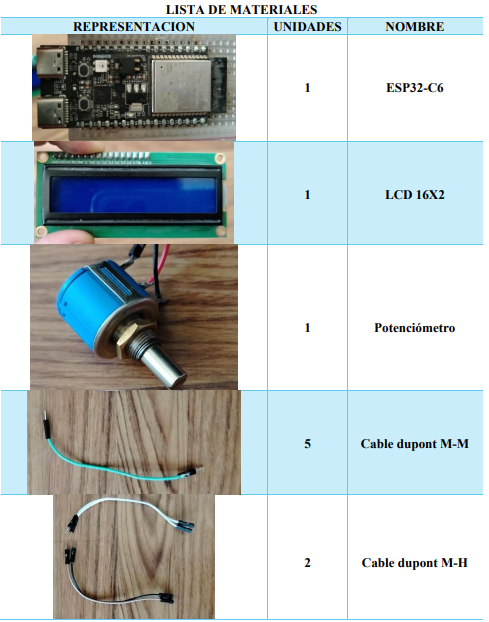
\includegraphics[trim = {0mm 0mm 0mm 0mm},clip,scale=0.5]{12/Img/listaDeMateriales1.png}
        \caption{Lista de materiales}
        \label{fig:listaDeMateriales1.png}
    \end{figure}
    
    \subsection{Procedimiento de ensamble}
    \begin{itemize}
        \item Paso 1. Conectar el multi contacto a una fuente de energía.
        \item Paso 2. Conectar el ESP32-C6 al protoboard.
        \item Paso 3. Conectar los pines de alimentación VCC y GND.
        \item Paso 4. Conectar el potenciómetro a la protoboard, y mediante los extremos del potenciómetro conectar ek VCC y GND,junto con la central del pin analogico del ESP32-C6.
        \item Paso 5.Conectar la LCD al protoboard junto con las resistencias y condensores, Luego los pines de datos de series (I2C) y los pines de control al ESP32.
        \item Paso 6. Conectar el cable USB-C al multi contacto que le brindara la energía al ESP32.
        \item Paso 7. Al realizar la acción con el potenciómetro verificar que este funcione y haga la lectura indicada. 
    \end{itemize}
    Mediante este proceso debemos adquirir los resultados necesarios hasta llegar al esperado, dado que en el ensamble se pueden cometer errores se debe tener una correcta documentación para percibir areas de mejora en el proceso.
        
    
    %Cada estrategia metodológica se establece acorde a cada objetivo, y por tanto deberá ser desglosada precisada y ordenada claramente. En consecuencia cada objetivo que se presentó en forma de verbo en infinitivo deberá determinar una estrategia en forma de adverbio. Ej. Desarrollar…Desarrollo. Son las actividades ordenadas que tienen como finalidad la prueba de la hipótesis. 
    
    %\begin{itemize}
        %\item Se debe establecer que se habrá de hacer, como, conque, y donde para obtener la información que permita probar la hipótesis.  
        %\item Se debe desglosar de acuerdo a los objetivos específicos. 
        %\item Se debe establecer una estrategia metodológica por cada objetivo específico. De manera simplista se podría decir que se cambia el verbo en infinitivo por su respectivo adverbio.
        %\item En cada objetivo se debe describir que método, que materiales y que equipo se usará para conseguirlo.
        %\item Se deben tener referencias Figura \ref{fig:lcd-16x2}.
    %\end{itemize}
    % 
    % 
    %\begin{figure}[H]
        %\centering
        %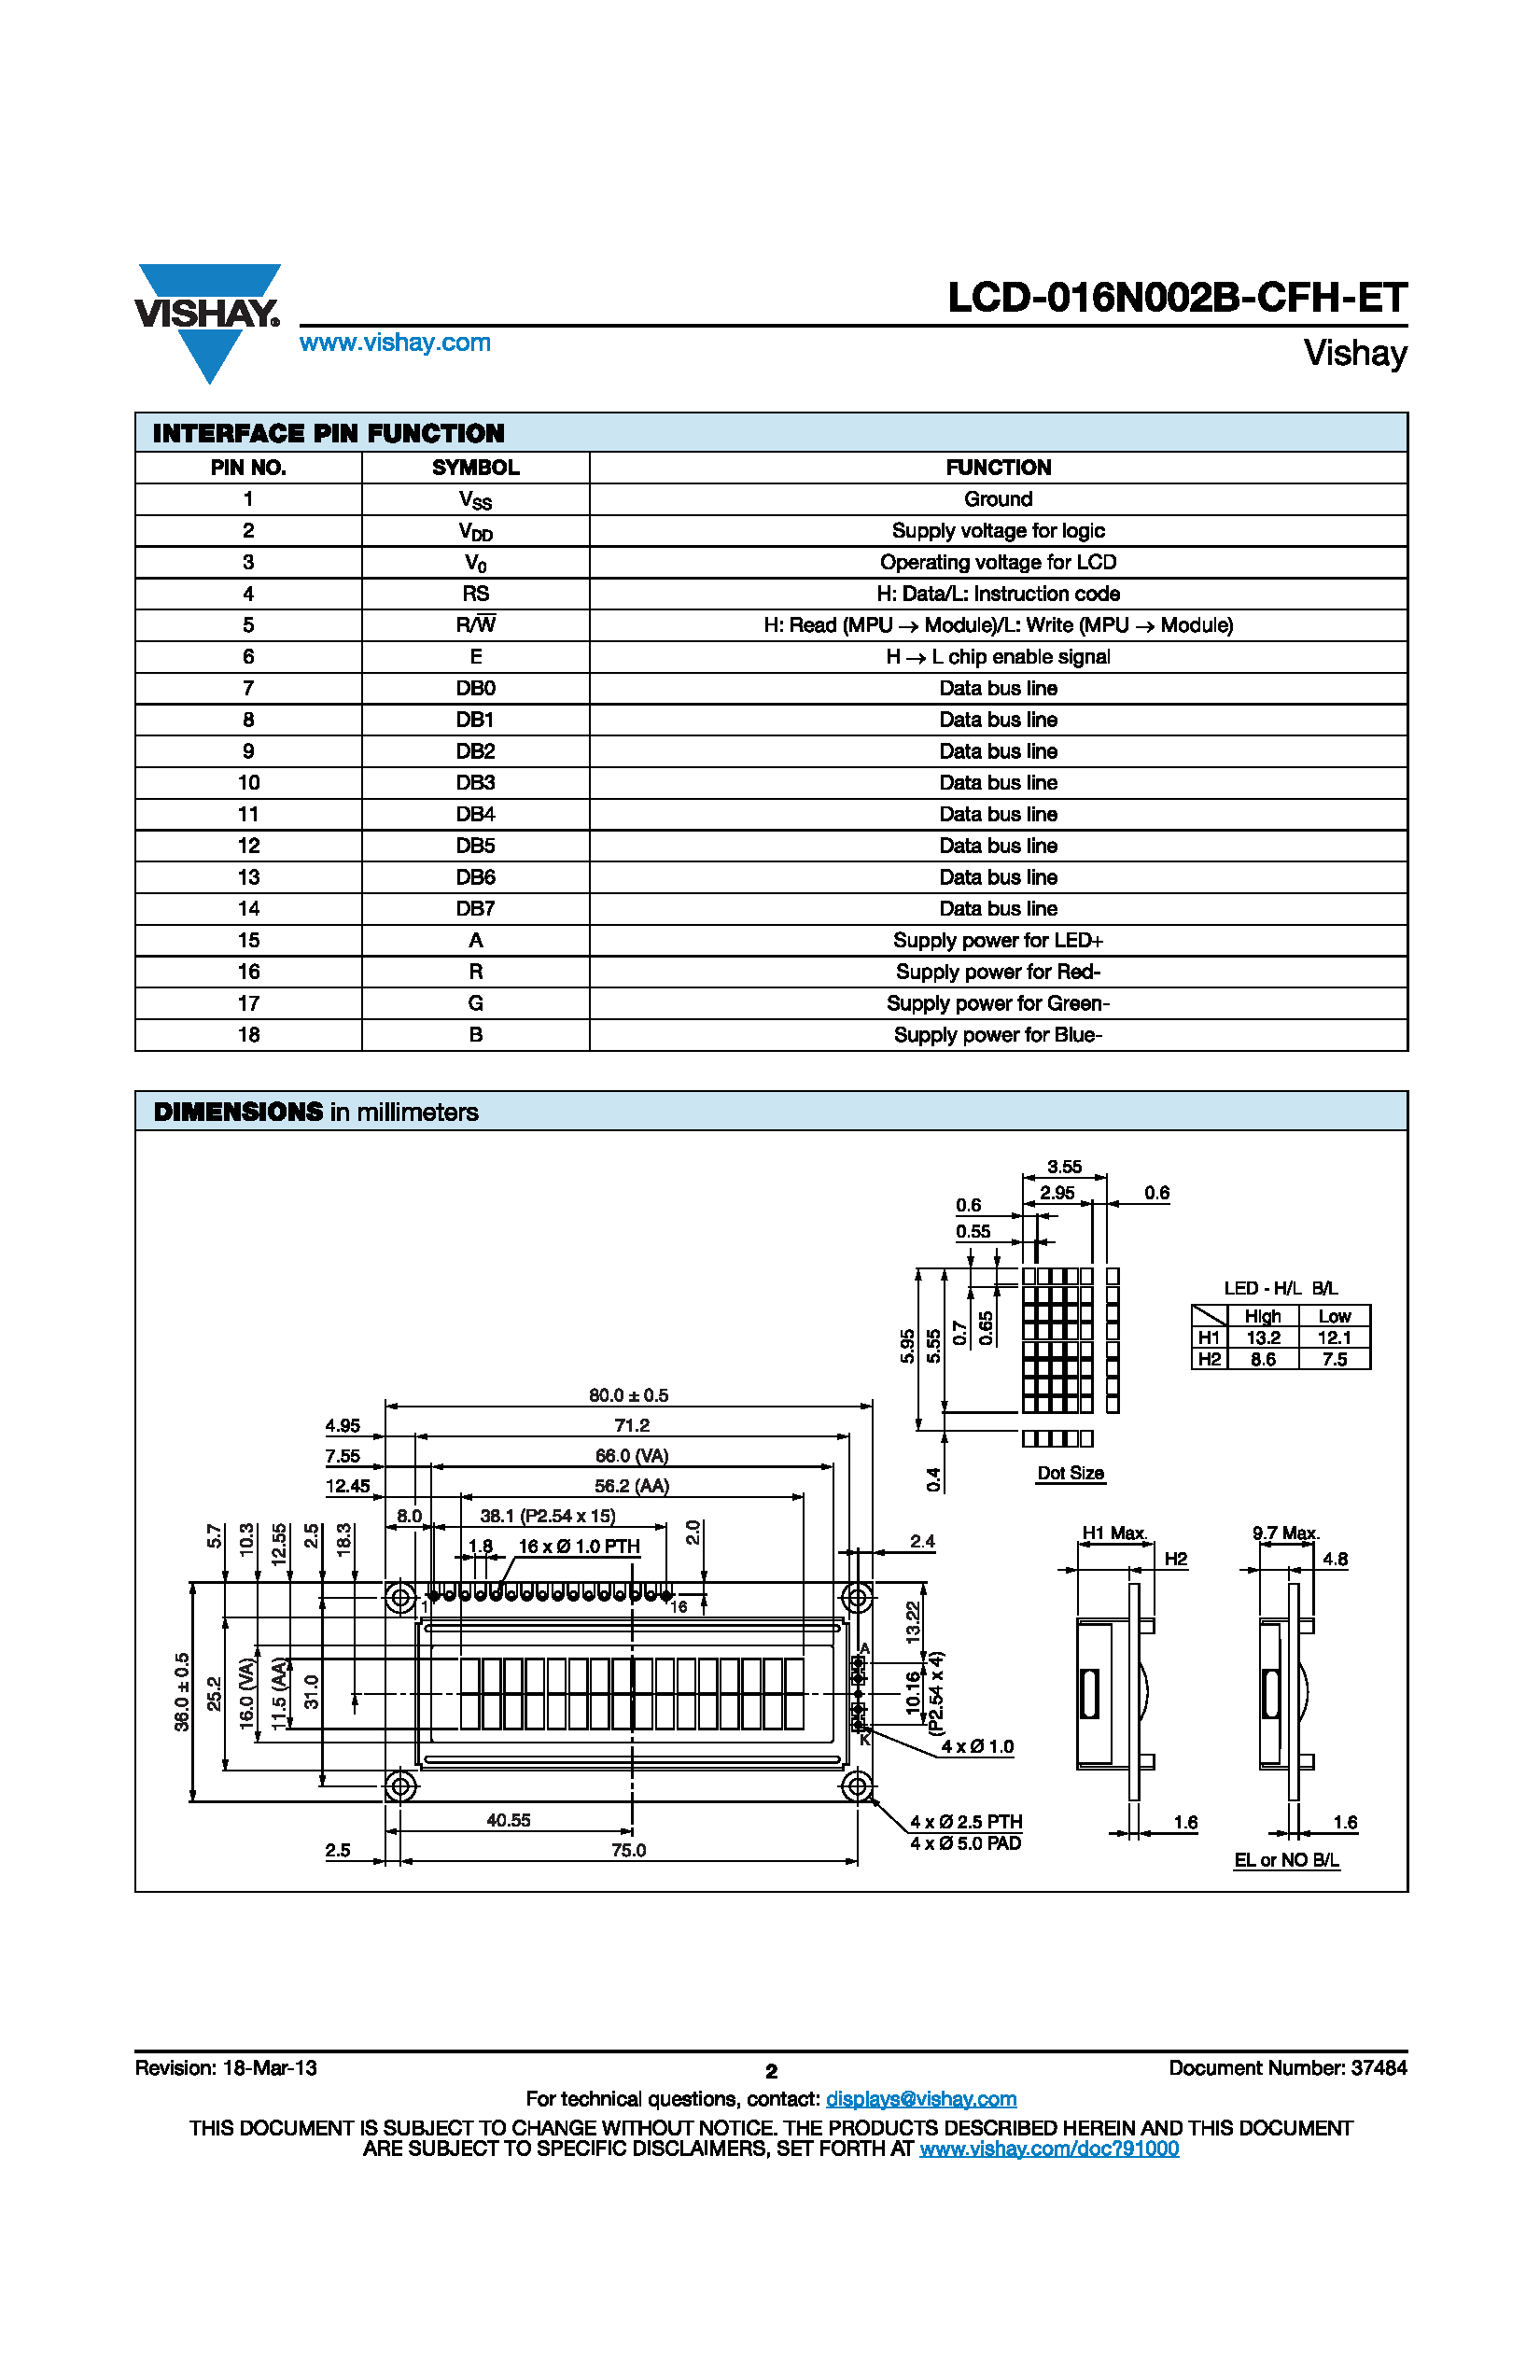
\includegraphics[trim = {30mm 65mm 90mm 250mm},clip,scale=0.5]{6/Img/lcd-16x2.pdf}
        %\caption{Esquema LCD de 16x2}
        %\label{fig:lcd-16x2}
    %\end{figure}
    % 
    % 
    %\begin{figure}[H]
        %\centering
        %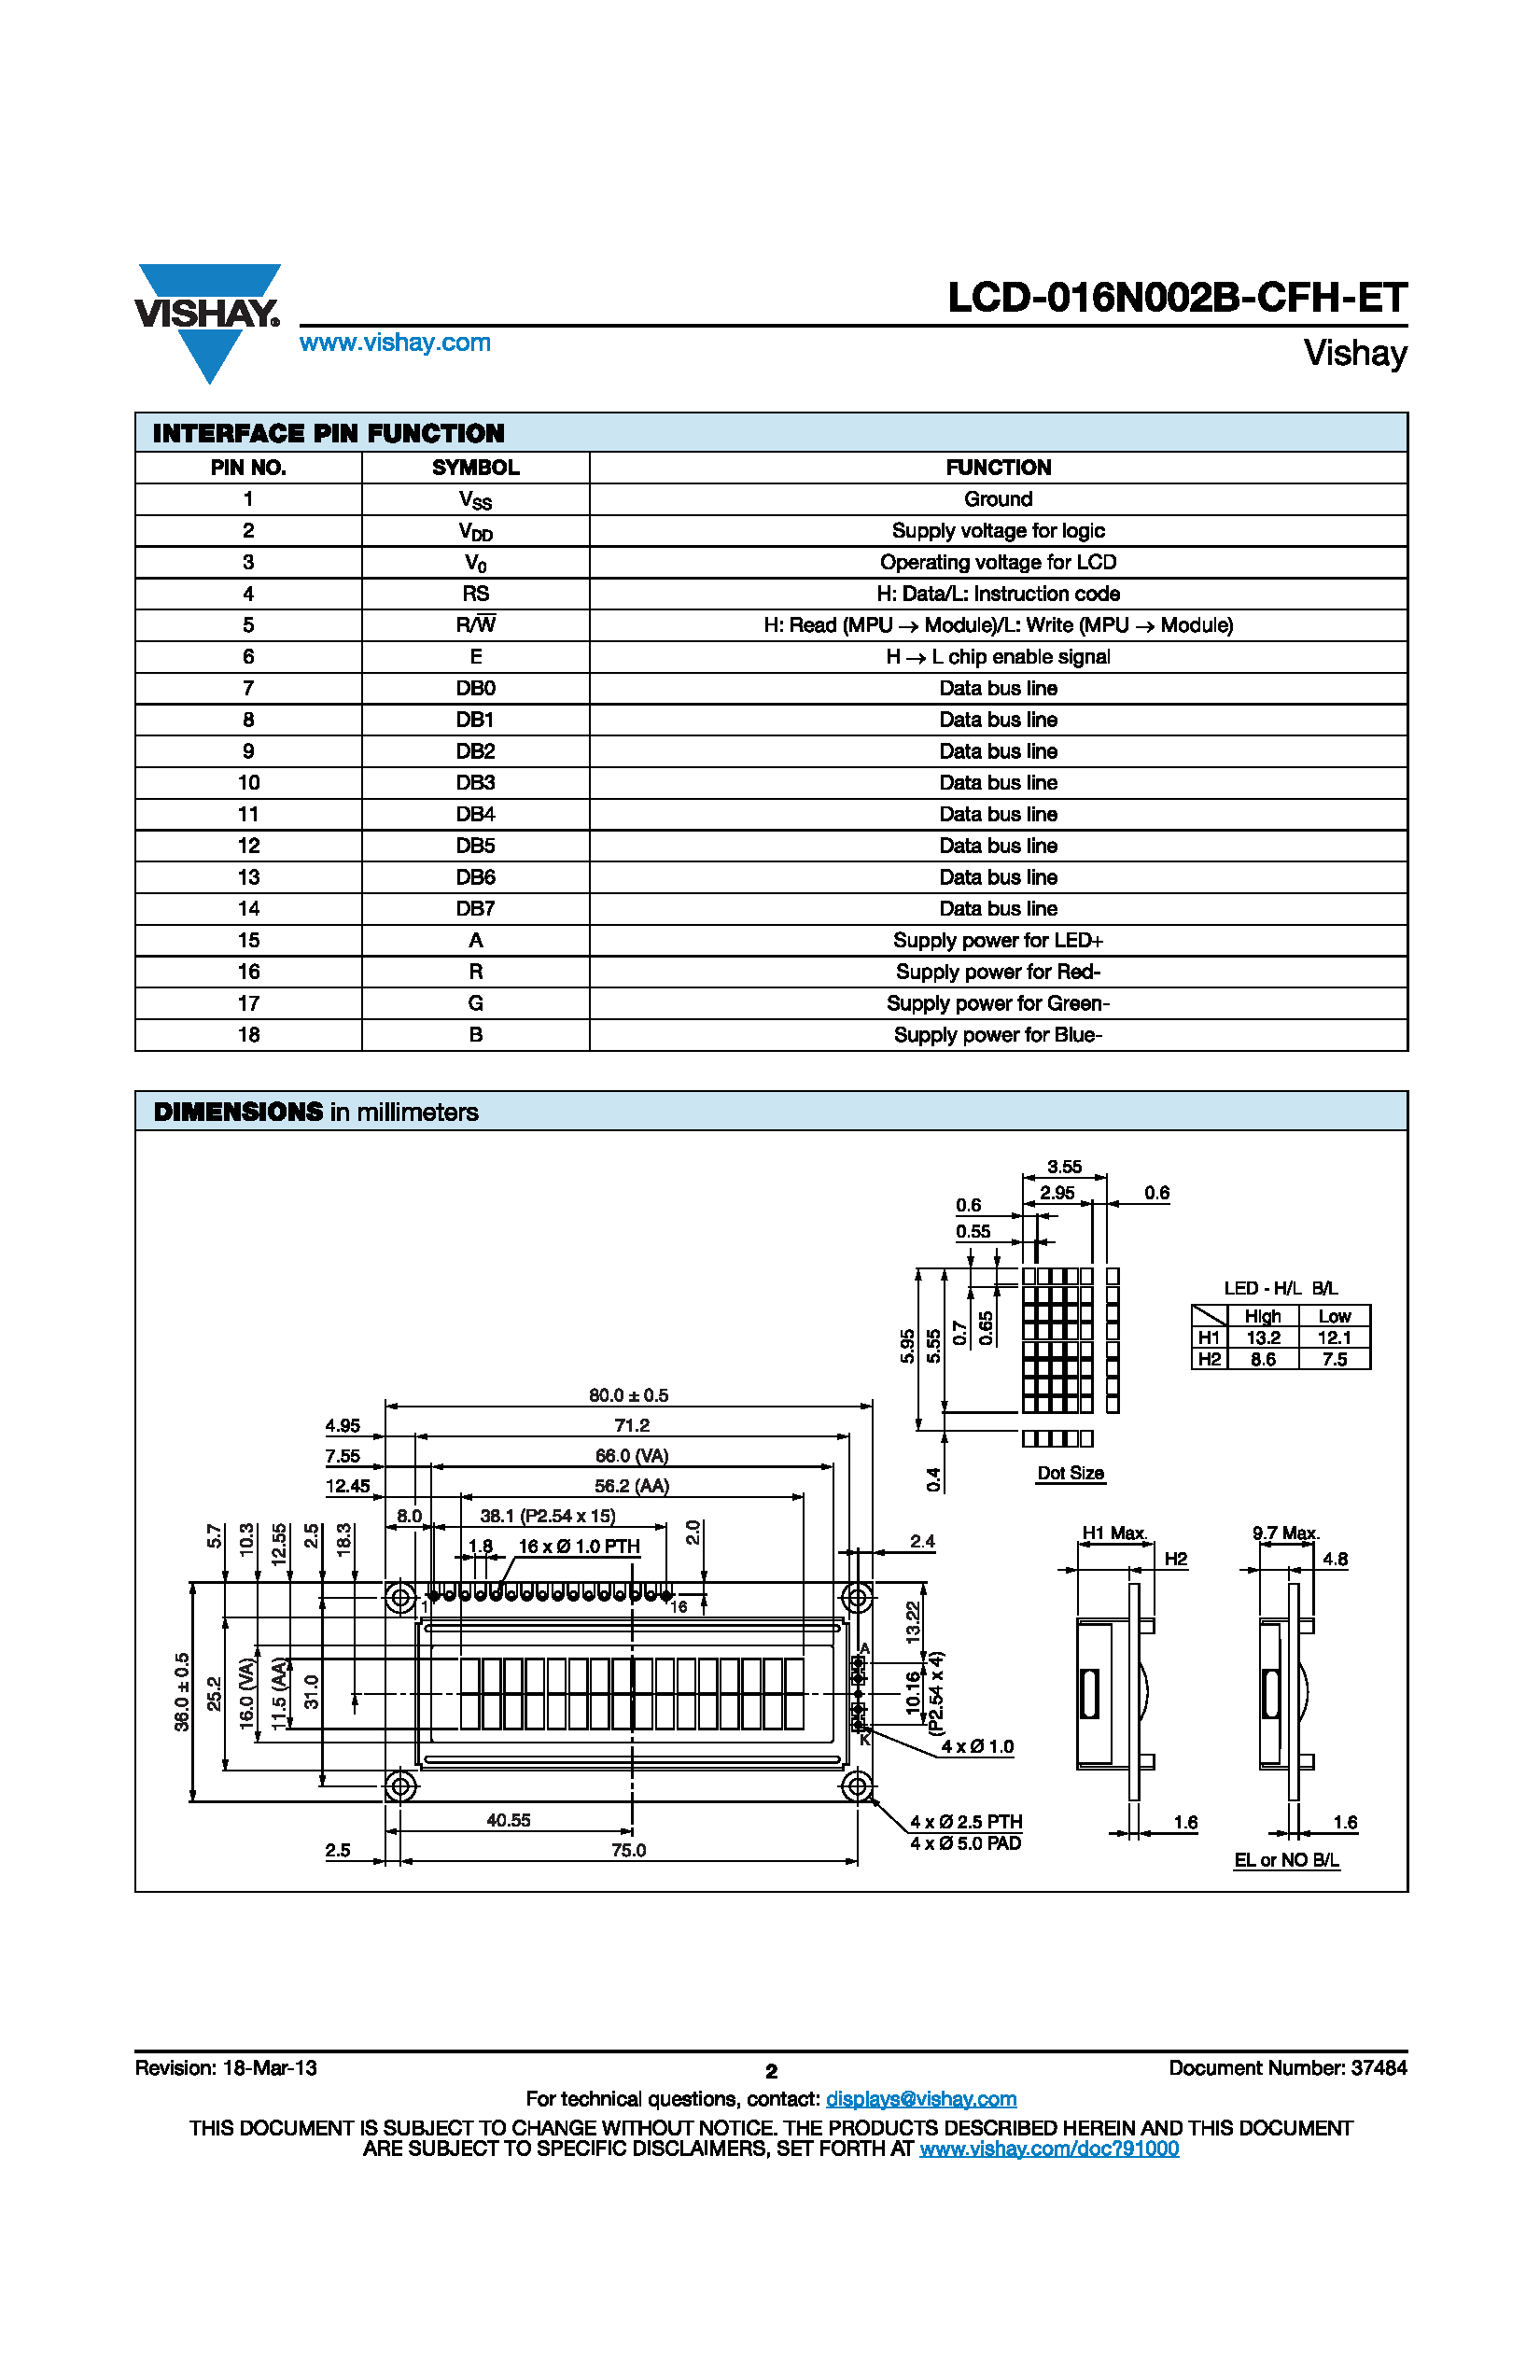
\includegraphics[trim = {30mm 250mm 90mm 20mm},clip,scale=0.5]{6/Img/lcd-16x2.pdf}
        %\caption{Esquema LCD de 16x2}
        %\label{fig:lcd-16x2}
    %\end{figure}
    % 
    % 
    \subsection{Prepara tu documento}
    
    Antes de que comiences a utilizar esta plantilla, es recomendable que prepare la información que contendrá en un archivo aparte. 
    Ten preparadas tus gráficas, así como también las tablas aparte, para que sea más fácil integrarlo. 
    Se recomienda fuertemente el uso de \textbf{formato Enhanced Metafile (.emf) para imágenes y gráficas} de resolución óptima. 
    Finalmente, completa y organiza el contenido antes de darle el formato de esta plantilla. 
    
    \subsection{Acrónimos y Abreviaciones}
    
    Los acrónimos y abreviaciones deberán ser definidos únicamente la primera vez que aparecen en el texto, esto para que el lector entienda lo que significan.
    
    \subsection{Ecuaciones}
    
    Las ecuaciones son una excepción a las especificaciones prescritas de esta plantilla. 
    Deberá determinar si su ecuación debe escribirse o no utilizando la fuente Adobe Devangari. 
    Para crear ecuaciones multinivel, puede ser necesario tratar la ecuación como un gráfico e insertarla en el texto después de aplicar el estilo de la platilla.
    Las ecuaciones serán enumeradas de manera consecutiva, y el número de ecuación, entre paréntesis, se colocan al ras de la derecha, utilizando una tabulación derecha. 
    
    \begin{equation}
        \label{eq1}
        x + y = z 
    \end{equation}
    
    Es importante asegurarse de que los símbolos de la ecuación sean definidos antes o inmediatamente después de la ecuación. Utilice “(1)”, en vez de “Eq. 1” al enumerar las ecuaciones, excepto al principio de una oración: “La ecuación (\ref{eq1}) es…”
    
    \section{Resultados y discusión}
    
    Antes de comenzar a preparar tu artículo, es importante que lea primero la guía del autor, la cual incluye los temas o apartados que son necesarios para tener tu trabajo completo.
    Una vez completada la edición del texto, el documento está listo para el uso de esta plantilla. En este archivo recién creado, resalte todo el contenido e importe el archivo de texto preparado. Ahora esta listo para estilizar su documento.
    En esta sección se deben presentar todo lo obtenido de la sección 2, incluidas deducciones o efectos del desarrollo. También se podrán incluir subsecciones numeradas de la siguiente forma:
    
    \subsection{Autores y Afiliaciones}
    
    Para distinguir las afiliaciones de los autores, utilice superíndices iniciando con el número 1, 2, etc., sucesivamente, esto dependerá de la cantidad de los departamentos a los que estén afiliados los autores. En caso de que todos los autores pertenezcan a una mismo departamento e institución, utilizar sólo el superíndice 1. 
    
    \subsection{Identificar los encabezados}
    
    Se les recuerda a los autores que los encabezados deben de estar conforme los solicita la guía del autor. De ahí se puede adaptar el trabajo para que sea más fácil de entender para el lector.
    Los encabezados organizan los temas sobre una base relacional y jerárquica. Por ejemplo, el título del documento es encabezado del texto principal porque todo el material posterior se relaciona y elabora sobre este tema. 
    
    \subsection{Tablas y Figuras}
    
    \begin{enumerate}
        \item Posición de las tablas y figuras: Coloque las figuras y las tablas en la parte superior e inferior de las columnas. Evite colocarlos en medio. Las figuras y las tablas grandes pueden abarcar ambas columnas. Los títulos de las figuras deben de estar debajo de las mismas; los títulos de las tablas deben aparecer encima de ellas. Insértese las figuras y los cuadros después de citarse en el texto. Utilice la abreviatura “Fig. 1”, incluso al principio de una oración. 
    \end{enumerate}
    
    \section{Conclusiones}
    
    Se describe aquí el alcance del trabajo, logros obtenidos y perspectivas para el futuro de este. Se sugiere colocar información cuantitativa obtenida.
    
    \section{Agradecimientos}
    
    Es importante darles su debido reconocimiento a los laboratorios, instituciones, organizaciones, entre otros que han sido participes para la culminación de este trabajo. También es importante mencionar, fondos, proyectos, becas, entre otros que se le han otorgado al o los autores para realizar el trabajo de investigación. Ejemplo: “Los autores agradecen al Concejo Nacional de Ciencia y Tecnología por los recursos otorgados…”
    
    \section*{Referencias}
    \cite{REF2}
    \cite{REF4}
    \cite{REF5}
    \cite{REF6}
    \cite{REF7}
    \cite{REF8}
    \cite{REF9}
    %Para esta platilla, se solicita al autor enumerar las citas de manera consecutiva entre corchetes \cite{YLi2013}. 
    %La puntuación de la oración que sigues sería \cite{Mesaelides2011}. 
    %Refiérase simplemente al número de referencia, como en \cite{Morales2012}, no utilice “Ref. [3]” o “referencia [3]” excepto al principio de una oración: “La referencia [3] fue la primera…”
    %Enumere las notas al pie por separado en superíndices. Coloque la nota de pie de en la parte inferior de la columna en la que se citó. No coloque notas al pie en la lista de referencias. Utilice letras para las notas al pie de la tabla.
    %A menos de que haya tres autores o más; no utilice “et al.”. Los trabajos que no hayan sido publicados, incluso si han sido presentados para su publicación, deben ser citados como “inéditos”. Los trabajos que han sido aceptados para su publicación deben de citarse como “en prensa”. Poner en mayúscula sólo la primera palabra de un título, excepto los nombres propios y los símbolos de elemento. 
    %Otros ejemplos \cite{LAAngeles2021}, \cite{LAAngelesConni}. 
    %Véase el archivo adjunto \ref{anexo:pines}.
    
    % Ejemplo
    %  @Article{article,
    % 	author = "Author1 LastName1 and Author2 LastName2 and Author3 LastName3",
    % 	title = "Article Title",
    % 	volume = "30",
    % 	number = "30",
    % 	pages = "10127-10134",
    % 	year = "2013",
    % 	doi = "10.3389/fnins.2013.12345",
    % 	URL = "http://www.frontiersin.org/Journal/10.3389/fnins.2013.12345/abstract",
    % 	journal = "Frontiers in Neuroscience"
    % }
    
    % @book{book,
    %   author    = {Author Name}, 
    %   title     = {The title of the work},
    %   publisher = {The name of the publisher},
    %   address   = {The city},
    %   year      = 1993,
    % }
    
    % @incollection{chapter,
    %   author       = {Bauthor Surname}, 
    %   title        = {The title of the work},
    %   editor       = {Editor Name},
    %   booktitle    = {The title of the book},
    %   publisher    = {The name of the publisher},
    %   address      = {The city},
    %   year         = 2002,
    %   pages        = {201-213},
    % }
    
    % @InProceedings{conference,
    %   author = {Cauthor Name and Dauthor Surname and Fauthor LastName},
    %   title = {The title of the work},
    %   booktitle = {The title of the conference proceedings},
    %   year = 1996,
    %   publisher = {The name of the publisher},
    %   editor = {Editor Name1 and Editor Name2},
    %   pages = {41-50},
    % }
    
    % @book{cho,
    %   author       = {Gauthor Name1}, 
    %   title        = {The title of the work},
    %   publisher = {Country code and patent number},
    %   address      = {Patent Country},
    %   year = 2013
    % }
    
    % @book{patent,
    %   author    = {Hauthor Surname1}, 
    %   title     = {The title of the work},
    %   publisher = {Patent number},
    %   address   = {Patent country},
    %   year      = 2010,
    % }
    
    % % please use misc for datasets
    % @misc{dataset, 
    % 	author = "Author1 LastName1 and Author2 LastName2 and Author3 LastName3",
    % 	title = "Data Title",
    % 	year = "2011",
    % 	doi = "10.000/55555",
    % 	URL = "http://www.frontiersin.org/",
    % }
    
    \bibliographystyle{ieeetr}
    \bibliography{12/referencias}
    % 
    % 
    %%%%%%%%%%%%%%%%%%%%%%%%%%%%%%%%%%
    \appendix
    %%%%%%%%%%%%%%%%%%%%%%%%%%%%%%%%%%
    % 
    % 
    \centering{\section[\appendixautorefname{}]{Apéndice}}\label{anexo:listaMateriales}
    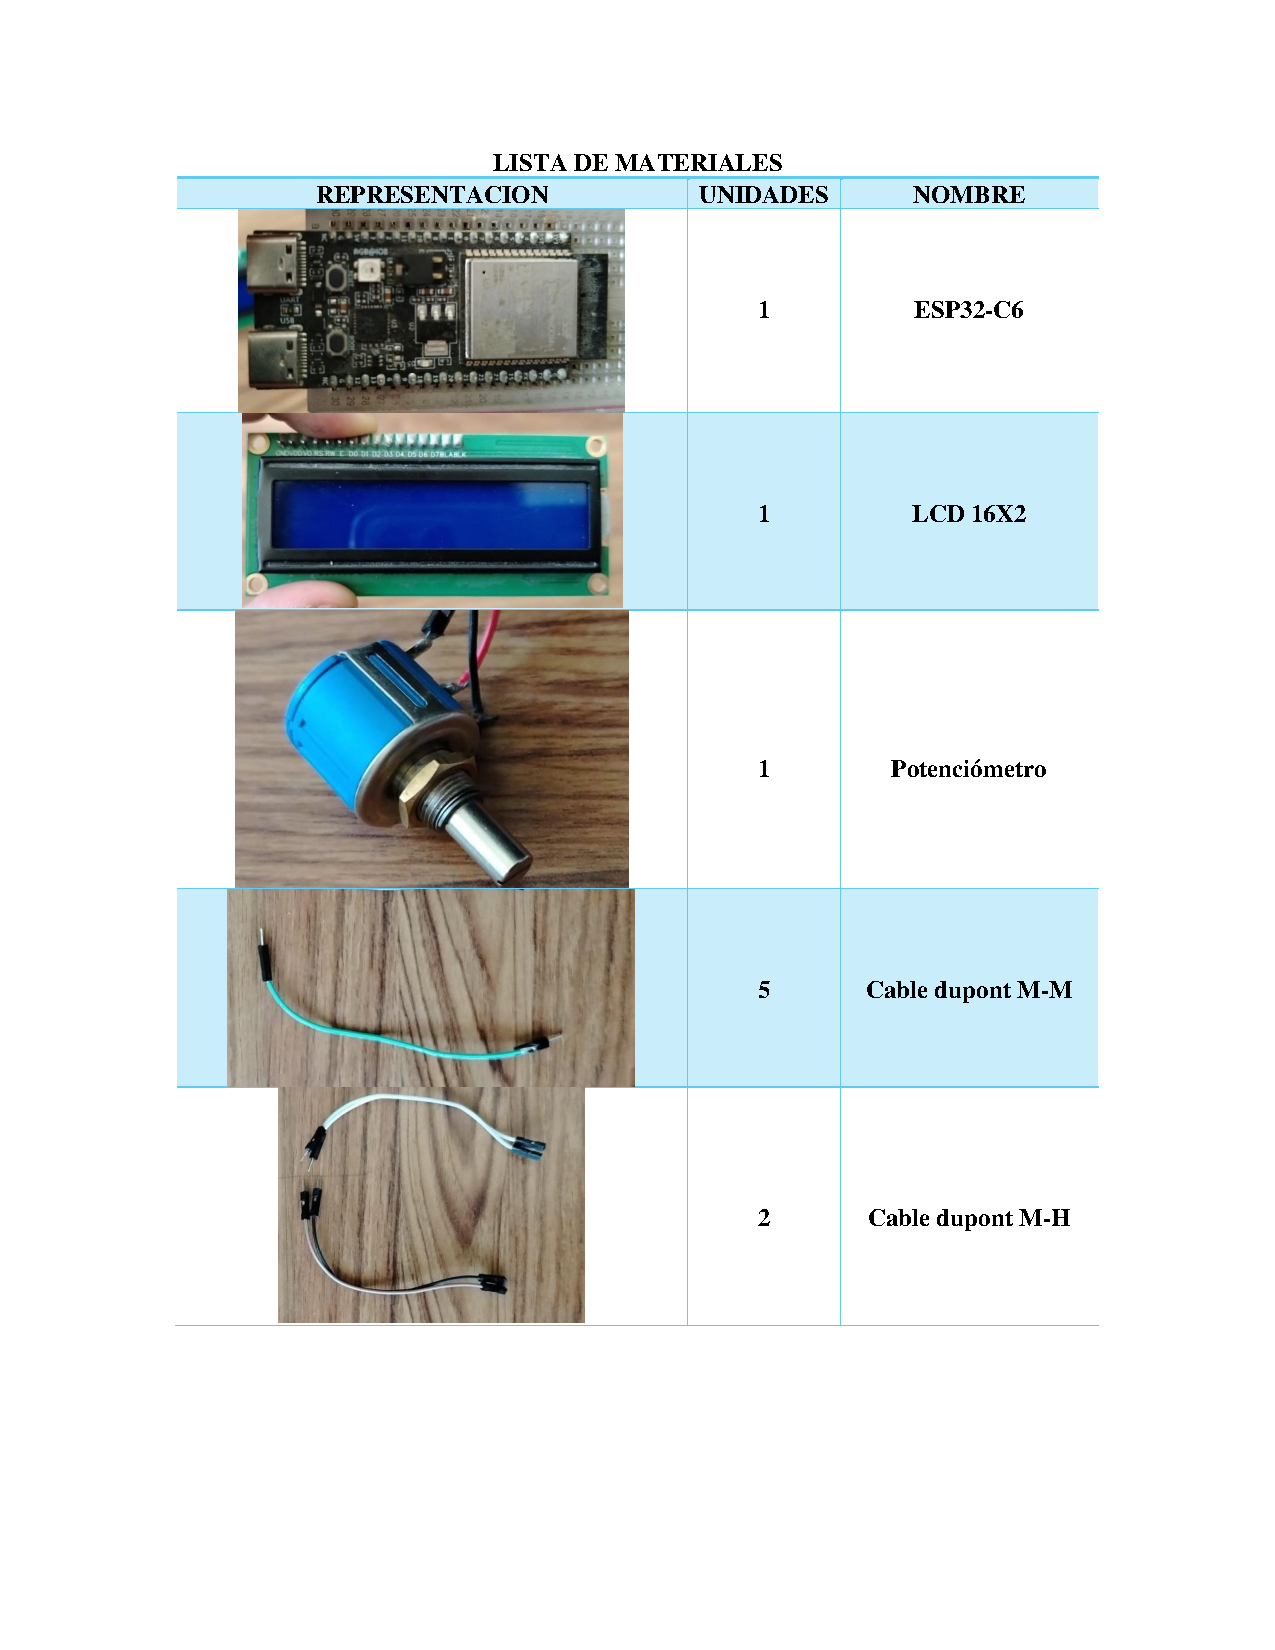
\includepdf[pages=-]{12/Img/listaMateriales.pdf}
    \centering{\section[\appendixautorefname{}]{Apéndice}}\label{anexo:guiaDeEnsamble}
    \includepdf[pages=-]{12/Img/guiaDeEnsamble.pdf}
    %%%%%%%%%%%%%%%%%%%%%%%%%%%%%%%%%%%%%%%%
    